\documentclass[hidelinks,letterpaper, 11pt]{article}
\usepackage{graphicx, bm, booktabs, lineno, array}
\usepackage[fleqn]{amsmath}
\usepackage{nicefrac}
\usepackage[numbers, super, sort&compress]{natbib}
\usepackage[right=1in, left=1in, top=1in, bottom=1in]{geometry}
\usepackage[parfill]{parskip}
\usepackage[usenames,dvipsnames]{color}
\usepackage[font=large,labelfont=bf,margin=1cm, labelsep = none]{caption}
\usepackage{setspace}
\usepackage{gensymb}
\usepackage{color}
\usepackage{sidecap}
\usepackage{etoolbox}
\usepackage{tcolorbox}
\usepackage{newpxtext,newpxmath}
\tcbuselibrary{breakable}
\newbool{MyRefNumbers}
\usepackage{authblk}
\usepackage{hyperref}
\usepackage{mathpazo}
\usepackage[color=cyan, textsize=tiny]{todonotes}
\usepackage[font={normalsize}]{caption}
\usepackage{adjustbox}
\usepackage{array}
\usepackage{booktabs}
\usepackage{multirow}
\usepackage{tabularx}

\setlength{\mathindent}{0pt}
\setlength{\parindent}{1cm}
\pdfminorversion=3

\newcommand*\samethanks[1][\value{footnote}]{\footnotemark[#1]}
\newcommand\blfootnote[1]{%
	\begingroup
	\renewcommand\thefootnote{}\footnote{#1}%
	\addtocounter{footnote}{-1}%
	\endgroup
}



\begin{document}
	
	
	
\doublespacing
\title{Water shifts the balance of coexistence}
\author[1, $\dagger$]{Po-Ju Ke}
\affil[1]{Institute of Ecology and Evolutionary Biology, National Taiwan University, Taipei, Taiwan}
\date{\today}
\maketitle
\blfootnote{$\dagger$ Correspondence author: Institute of Ecology and Evolutionary Biology, National Taiwan University, Taipei 10617, Taiwan. Phone: +886 02-3366-2467. Email: pojuke@ntu.edu.tw}
	
\onehalfspacing
\noindent \textbf{Type of article:} News \& Views\\
\noindent \textbf{Subject strapline:} Plant--soil feedback\\
\noindent \textbf{Words in main text:} 1000\\
\noindent \textbf{Number of figures:} 1\\
\noindent \textbf{References:} 12\\
\noindent \textbf{Author ORCID:} 0000-0002-8371-7984\\
	

\linenumbers
\doublespacing


\newpage
\section*{Standfirst}
\textbf{Experimentally manipulating precipitation levels in a plant-soil feedback experiment reveals changes to the interactions between plants and soil microbes that render community dynamics less predictable under wetter conditions.}
%Experimentally manipulating precipitation levels reveals diversity-eroding plant--soil feedbacks under wetter conditions that render plant community dynamics less predictable.
\bigskip



\section*{Main text}
% Openning
The soil that plants grow in harbors a diverse array of soil microbes that can affect plant growth \citep{vanderPutten2013}. 
Recent research has highlighted that the interactions between plants and soil microbes can vary with environmental factors such as nutrient and water availability \citep{Smith2017, DeLong2019}.
Such context dependency makes it challenging to predict the consequence of plant--soil microbe interactions, but understanding it is of increasing importance as climate change introduces variation in environmental factors across time \citep{Pugnaire2019}.
Writing in this issue of \textit{Nature Ecology \& Evolution}, Dudenh{\"o}ffer and colleagues \citep{Dudenhoffer2022} combine greenhouse experiments, high-throughput sequencing, and ecological modeling to show how soil water content alters the community-level consequences of plant--soil microbe interactions. 
\medskip


% Background of the field -- Bever's PSF framework
In the ecological literature, the plant--soil feedback (PSF) theory \citep{Bever1997} highlights that soil microbes can affect plant communities by generating frequency-dependent feedback loops, with overall impacts on plant coexistence that can be predicted by a theory-derived pairwise PSF metric.
Under the original two-species framework, negative pairwise PSF can occur when both plants condition their microbial communities to favor heterospecifics over conspecifics (Fig.~\ref{fig:PSFconceptual}a, left panels). 
When this happens, soil microbes drive negative frequency dependence that increases the tendency of different plant species to coexistence (Fig.~\ref{fig:PSFconceptual}b, left panels). 
Conversely, positive pairwise PSF can occur when plants condition microbial communities that favor conspecifics over heterospecifics (Fig.~\ref{fig:PSFconceptual}a, right panels), which destabilizes plant coexistence by favoring the initially abundant plant species (Fig.~\ref{fig:PSFconceptual}b, right panels).
However, these biotic interactions do not exist in isolation, but may be modulated by abiotic context. 
While previous studies have investigated the impact of soil water content on plant--soil microbe interactions, they have not yet leveraged existing theory to make predictions on plant coexistence.
\medskip 

% What the authors did in this study and results from greenhouse experiments
Dudenh{\"o}ffer and colleagues now fill this gap by conducting a multi-species water-manipulation experiment using PSF theory. 
Their impressive full factorial experiment used eight coastal prairie plant species, where each species is grown in sterile soil inoculated with `conditioned' soil from either the same species, or a different species, in order to transplant their respective microbial community and measure subsequent plant performance in the `response' phase.
All 64 plant species $\times$ soil type combinations were then grown under three watering treatments corresponding to extremely high, extremely low, or average local conditions.
To provide a holistic prediction of PSF under climate change, the authors imposed the watering treatment onto both the conditioning and the response phase of the experiment.
They found compelling evidence of a shift from coexistence-stabilizing negative pairwise PSF under drier conditions to coexistence-destabilizing positive pairwise PSF under wetter conditions (Fig.~\ref{fig:PSFconceptual}).
\medskip


% What's special -- New way to calculate the pairwise PSF index
Dudenh{\"o}ffer and colleagues develop a novel approach to integrate seedling survival into the calculation of pairwise PSF.
Previous studies mostly calculated the pairwise PSF metric based on measurements of plant biomass production in different soils \citep{Crawford2019}.
However, soil microbes can affect various aspects of plant performance throughout a plant's life span \citep{Dudenhoffer2017}.
While studies may also monitor seedling survival, the results are often presented as an additional microbial effect independent of biomass production.
In this study, plant mortality and biomass production of the surviving plants were fitted to different statistical distributions and the model coefficients used to estimate a plant species' average performance in different soils. 
The pairwise PSF metric calculated from these estimates compounds the effect of microbes on plant survival and biomass production, thereby unifying multiple microbial effects when predicting the context dependency of PSF. 
\medskip


% What's special -- IBM focusing on predictability
In order to further explore the likely long-term consequences of climate change-induced alterations to precipitation regimes, Dudenh{\"o}ffer and colleagues then parameterize a spatially-explicit model with their experimental data. 
These simulations predict that plant communities retain lower diversity and become less predictable under wetter conditions as positive pairwise PSF becomes more prevalent.
The latter is an important signature of positive pairwise PSF that is often overlooked: diversity is lost under such scenarios not because soil microbes confer a competitive advantage to a specific plant \citep{Kandlikar2019}, but because they drive priority effects (i.e., small random differences in initial species abundances would be amplified).
Interestingly, further explorations revealed that the context dependency of PSF can have complicated consequences on plant community assembly, with patterns depending on plant mortality, the spatial scale of PSF, and the number of plant species directly favored by positive microbial effects \citep{Kandlikar2019}. 
\medskip


% Limitations
Attributing the observed changes in PSF to specific shifts in microbial community composition, however, remains a non-trivial task. 
Common approaches usually involve searching for statistical relationships between differences in microbial composition and PSF strength and assigning probable functional guides to the metabarcoding data \citep{Nguyen2016}.
However, precisely due to context dependency, the same microbial community may have different impacts on plant performance in different soil watering treatments.
While challenging, future studies can use approaches such as metatranscriptomics to obtain further functional information, as well as single taxa or synthetic community bioassay to cement causal relationships.
\medskip


% Outlook for climate change
In the near future, we expect to see not only changes in mean precipitation magnitude but also changes in its temporal variability under climate change.
Moving forward requires knowledge on how the temporal aspects of PSF (e.g., the rate of soil conditioning and the rate at which plant responsiveness varies with ontogeny) interact with the frequency of wet--dry fluctuations and extreme events \citep{Rudgers2020, Ke2021}. 
For example, a change in the timing of drought may perturb the microbial succession trajectory at various stages and lead to distinct microbial legacies. 
Changes in the frequency of precipitation fluctuations may also influence how plants respond to soil microbes depending on the water availability during different plant ontogenetic stages.
To this end, greenhouse experiments subjecting only the conditioning or response phase of PSF to varying environmental contexts can provide valuable mechanistic insight.
Here, Dudenh{\"o}ffer and colleagues provided a solid baseline prediction upon which more complicated manipulations can be performed.
Together with latest development in PSF theory \citep{Kandlikar2019}, we are advancing towards robust prediction of how soil microbes affect plant community diversity, stability, and productivity in a changing world.
\bigskip



\clearpage
\begin{figure}[h]
	\vspace{-1.5cm}
	\centering
	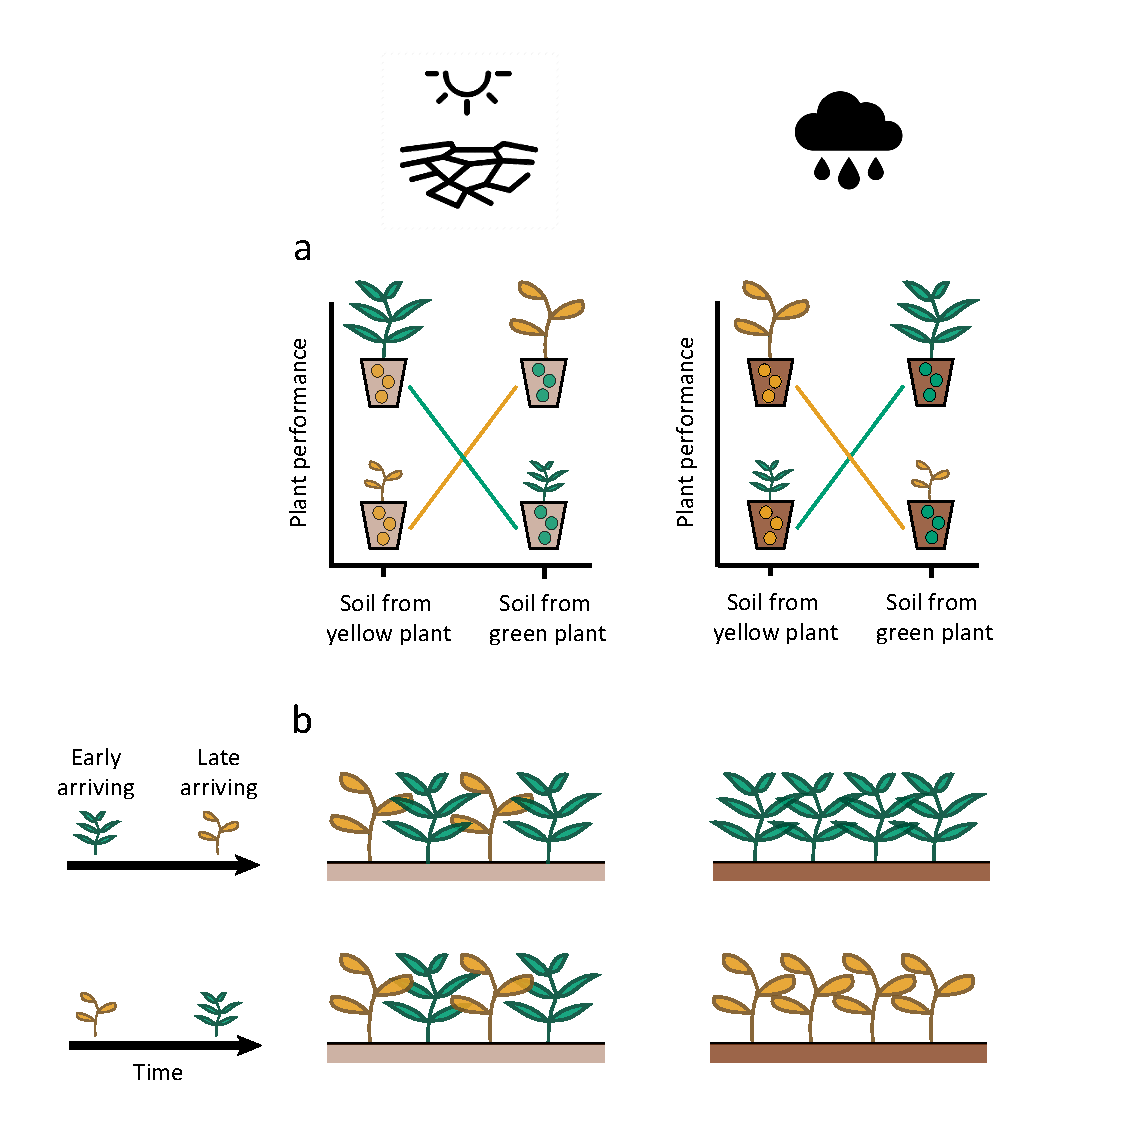
\includegraphics[width=0.75\linewidth]{../Figures/Figure1_ver6}
	\caption{\, \textbf{Plant--soil feedback under different precipitation level}. 
	\textbf{a}, Quantifying pairwise plant--soil feedback (PSF) with a transplant experiment. 
	Soils with different history are prepared by allowing the yellow and green plant to condition their species-specific soil microbial community (i.e., the conditioning phase), indicated by yellow and green circles, respectively. 
	Then, seedlings of the yellow and green plants are transplanted into soils conditioned by conspecifics and heterospecifics (i.e., the response phase), indicated by the match and mismatch between plant and microbe colors, respectively. 
	In this illustrative figure, the x-axis represents soils with different conditioning history and the y-axis represents plant performance, which is also indicated by the size of the plant icon.
	Negative pairwise PSF can occur when both plants condition their microbial community such that they perform worse in conspecific soils relative to the performance of the other species (left); positive pairwise PSF can occur when the opposite is true (right).
	\textbf{b}, Predicted plant competitive outcome under different PSF scenarios. 
	Negative pairwise PSF increases the tendency of plant coexistence (left), whereas positive pairwise PSF increases the tendency of priority effects (i.e., the competitive outcome depends on plant arrival order, which is indicated by the black arrow; right).
	% Note that the pairwise PSF index \citep{Bever1997} represents a necessary but not sufficient criterion for plant coexistence, and a recent study \citep{Kandlikar2019} has derived an additional metric for a more robust prediction of plant coexistence.
	Dudenh{\"o}ffer and colleagues \citep{Dudenhoffer2022} conducted a PSF experiment where they subjected both the conditioning and response phase to different watering treatments, indicated here with different shadings of brown. 
	Their results suggest a shift from negative pairwise PSF under drier conditions (left \& light brown) to positive pairwise PSF under wetter conditions (right \& dark brown).}	
	\label{fig:PSFconceptual} 
\end{figure}



\clearpage
\begin{thebibliography}{12}
	\bibitem{vanderPutten2013}
	van~der Putten, W.~H., Bardgett, R.~D., Bever, J.~D., Bezemer, T.~M., Casper,
	B.~B., Fukami, T., Kardol, P., Klironomos, J.~N., Kulmatiski, A., Schweitzer,
	J.~A., Suding, K.~N., van~der Voorde, T. F.~J., and Wardle, D.~A.
	\newblock {\em Journal of Ecology}{ \bf 101}(2), 265--276 (2013).
	
	\bibitem{Smith2017}
	Smith-Ramesh, L.~M. and Reynolds, H.~L.
	\newblock {\em Journal of Vegetation Science}{ \bf 28}(3), 484--494 (2017).
	
	\bibitem{DeLong2019}
	De~Long, J.~R., Fry, E.~L., Veen, G., and Kardol, P.
	\newblock {\em Functional Ecology}{ \bf 33}(1), 118--128 (2019).
	
	\bibitem{Pugnaire2019}
	Pugnaire, F.~I., Morillo, J.~A., Pe{\~n}uelas, J., Reich, P.~B., Bardgett,
	R.~D., Gaxiola, A., Wardle, D.~A., and Van Der~Putten, W.~H.
	\newblock {\em Science Advances}{ \bf 5}(11), eaaz1834 (2019).
	
	\bibitem{Dudenhoffer2022}
	Dudenh{\"o}ffer, J.-H., Luecke, N.~C., and Crawford, K.~M.
	\newblock {\em Nature Ecology \& Evolution}{ \bf } (2022).
	
	\bibitem{Bever1997}
	Bever, J.~D., Westover, K.~M., and Antonovics, J.
	\newblock {\em Journal of Ecology}{ \bf 85}(5), 561--573 (1997).
	
	\bibitem{Crawford2019}
	Crawford, K.~M., Bauer, J.~T., Comita, L.~S., Eppinga, M.~B., Johnson, D.~J.,
	Mangan, S.~A., Queenborough, S.~A., Strand, A.~E., Suding, K.~N., Umbanhowar,
	J., et~al.
	\newblock {\em Ecology Letters}{ \bf 22}(8), 1274--1284 (2019).
	
	\bibitem{Dudenhoffer2017}
	Dudenh{\"{o}}ffer, J., Ebeling, A., Klein, A., Wagg, C., and Farrer, E.
	\newblock {\em Journal of Ecology}{ \bf 106}(1), 230--241 (2018).
	
	\bibitem{Kandlikar2019}
	Kandlikar, G.~S., Johnson, C.~A., Yan, X., Kraft, N.~J., and Levine, J.~M.
	\newblock {\em Ecology Letters}{ \bf 22}(8), 1178--1191 (2019).
	
	\bibitem{Nguyen2016}
	Nguyen, N.~H., Song, Z., Bates, S.~T., Branco, S., Tedersoo, L., Menke, J.,
	Schilling, J.~S., and Kennedy, P.~G.
	\newblock {\em Fungal Ecology}{ \bf 20}, 241 -- 248 (2016).
	
	\bibitem{Rudgers2020}
	Rudgers, J.~A., Afkhami, M.~E., Bell-Dereske, L., Chung, Y.~A., Crawford,
	K.~M., Kivlin, S.~N., Mann, M.~A., and Nu{\~n}ez, M.~A.
	\newblock {\em Annual Review of Ecology, Evolution, and Systematics}{ \bf 51}, 561--586 (2020).
	
	\bibitem{Ke2021}
	Ke, P.-J., Zee, P.~C., and Fukami, T.
	\newblock {\em New Phytologist}{ \bf 231}(4), 1546--1558 (2021).
\end{thebibliography}



\section*{Competing interests}
The author declare no competing financial interests.



\end{document}



